\documentclass[tikz]{standalone}
\usetikzlibrary{matrix, ext.positioning-plus}
\tikzset{% https://tex.stackexchange.com/a/660100/16595
  columns/.style 2 args={/utils/tempa/.style={column ##1/.append style={#2}},/utils/tempa/.list={#1}},columns*/.style 2 args={columns={#1}{nodes={#2}}},
  rows/.style 2 args={/utils/tempa/.style={row ##1/.append style={#2}},/utils/tempa/.list={#1}},rows*/.style 2 args={rows={#1}{nodes={#2}}}}
\tikzset{ 
  common/.style={
    text depth=1.25ex, text height=2.5ex,     
    inner ysep=+0pt, draw=black,
    align=center,
    text width=width("Brake")-4*(\pgfkeysvalueof{/pgf/inner xsep}),
  },
  common'/.style={
    common, align=right, text width=width("$-0.00$")},
  table/.style={
    nodes=common, matrix of math nodes,
    every outer matrix/.append style={inner sep=+0pt},
    row sep=-\pgflinewidth, column sep=-\pgflinewidth, nodes in empty cells},
}
\begin{document}
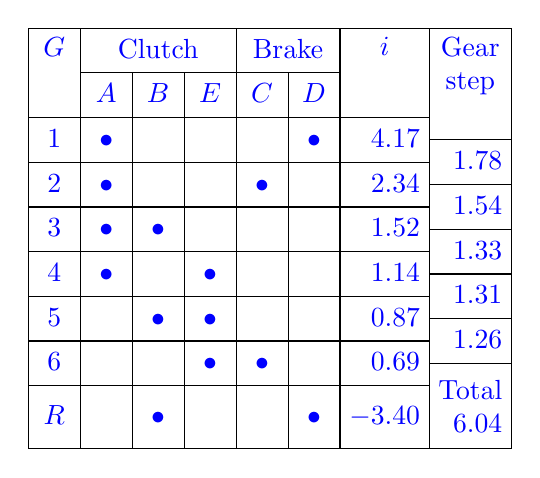
\begin{tikzpicture}[blue]
\matrix at (11,-3.5) (mat1) [
  table,
  columns*={7}{common'},
  rows*={8}{inner ysep=.3333em}
]{
  \path; & A       & B       & E       & C       & D  & \path; \\
  1 & \bullet &         &         &         & \bullet &  4.17 \\
  2 & \bullet &         &         & \bullet &         &  2.34 \\
  3 & \bullet & \bullet &         &         &         &  1.52 \\
  4 & \bullet &         & \bullet &         &         &  1.14 \\
  5 &         & \bullet & \bullet &         &         &  0.87 \\
  6 &         &         & \bullet & \bullet &         &  0.69 \\
  R &         & \bullet &         &         & \bullet & -3.40 \\
};
\path[
  node distance=-\pgflinewidth,
  l/.style={l'={$##1$}},
  l'/.style={label={[anchor=north, align=center]north:{##1}}},
  common''/.style={common', text width=width("Total")}]
  {[common/.append style={text width=}] % suppress overfull hboxes
    node[common, above=of -(mat1-1-2)(mat1-1-4)] (mat1-0) {Clutch}
    node[common, above=of -(mat1-1-5)(mat1-1-6)] {Brake}
  }
  node[right=of |(mat1-0)(mat1-1-6), common', l=i] (mat1-i) {}
  node[left=of |(mat1-0)(mat1-1-2), common, l=G] (mat1-G) {}
  foreach \Val [count=\vAl from 2, count=\vaL from 3] in {1.78, 1.54, 1.33, 1.31, 1.26}{
    node[
      common'',
      right=of (mat1-\vAl-7)(mat1-\vaL-7),
    ] (mat1-\vaL-8) {\Val}
  }
  node[
    common'',
    text height=, text depth=,
    right={of |([yshift=\pgflinewidth]mat1-7-8.south west)(mat1-8-7)}
  ] {Total\\6.04}
  node[
    common'',
    text height=, text depth=,
    align=center,
    right={of |([yshift=-\pgflinewidth]mat1-3-8.north west)(mat1-i)},
    l'={Gear\\step},
  ] {}
;
\end{tikzpicture}
\end{document}